\documentclass[11pt]{article}
\usepackage{geometry, url, amsmath, amssymb, algorithm, algpseudocode, soul, xcolor, graphicx}

\geometry{a4paper, scale=0.8}
\newtheorem{theorem}{Theorem}

\title{ARPA Network Whitepaper}
\author{Penrose}
\date{\today}

\begin{document}

\maketitle

\begin{abstract}
(Abstract is undone, feel free to add or comment) ARPA Network provides an efficient, permissionless threshold signature service for blockchains. At its core, the ARPA Network contains a threshold BLS signature that meets the need for decentralization, non-interactiveness, verifability, and high availability. The design and implementation of the network are premised on enhancing the blockchain and providing the threshold signature capability for users. Finally, Randcast is proposed as a distributed random number generator as a use case of the ARPA network. 

\end{abstract}

\section{Introduction}
As a distributed global ledger, the blockchain has proven its great significance of being an infrastructure of cyberspace. During the past decade, academic and industrial experts have made extensive efforts to improve its privacy, scalability, and interoperability. An effective means to enhance the blockchain is by verifiably outsourcing on-chain computation and storage to off-chain through threshold cryptography schemes. These schemes offer trust by their provable security and decentralization, which matches the distributed and trustless nature of the blockchain. At the same time, the blockchain can, as a bulletin board, serve as a reliable broadcast channel for these cryptographic algorithms. Therefore, combining threshold cryptography with blockchains can simultaneously strengthen blockchains and facilitate the implementation of threshold cryptography.

In this paper, we propose ARPA Network, a permissionless distributed network to provide essential threshold signature capability for blockchains. Roughly speaking, threshold signature is a protocol processing signature-related functions among a group of nodes through multi-party computation (MPC). It can help keep secrets distributedly, reach consensus by a majority vote, or hide the identity of signers. With the aid of the ARPA Network, one can build applications regrading secure key management, anonymous transaction, cross-chain messaging, quorum approval, distributed randomness generation, etc. Like the blockchain, the trust of the ARPA Network comes from the distribution across independent nodes. Those nodes are grouped and execute the threshold Boneh–Lynn–Shacham (BLS) signature scheme. Thanks to the aggregatability of BLS signatures and the node management mechanism we apply, the ARPA Network has the following features.
\begin{itemize}
    \item Decentralization, ARPA nodes provide threshold signature service in a decentralized manner. Trust is distributed to multiple entities located in different regions running individual nodes. This manner offers better tamper-proof in the physical level.
    \item Flexibility, ARPA protocol supports a variety of signature applications. Users are allowed to customize their signature policy, import or export secrets, and choose the security level
    \item Verifiability, ARPA signature scheme allows users to trivially verify their signatures. By virtue of the underlying cryptographic primitive, The signatures are unlikely to be forged or manipulated
    \item Non-interactivity, ARPA protocol avoids heavy synchronous communication in the signature generation phase. A non-interactive procedure guarantees reliable service status and flexible network topology.
    \item High availability, ARPA signature service keeps a high availability thanks to its decentralization and non-interactivity. With the growth of its network size, the downtime will reduce accordingly.
    \item Multiple Chain Supported, ARPA network is designed to adapt to multiple chains, facilitating developers from multiverse building their applications. Our underlying threshold signature network may keep consistency between the different data replicas.
\end{itemize}

In the remainder of this paper, we first overview the existing threshold signature schemes and point out the reason why threshold BLS signature is suitable for distributed systems in section 2. Then section 3 lists out presuppositions and the building blocks of our design. A walk-through of our implemented protocol is given in section 4, including the cryptographic part and the node management mechanism. And section 5 presents the system design by showing the high-level architecture of the network. Finally, section 6 demonstrates Randcast, a distributed pseudo-random number generator as a use case of the ARPA Network.

\section{Background and Related Works}

Threshold signature has been researched and applied extensively in the last few years. Many classical signature algorithms have been thresholdized, including BLS, ECDSA \cite{gennaro2018fast}, EdDSA \cite{stinson2001provably}, RSA \cite{damgaard2001practical}. However, when applied to a distributed system, not all threshold signature schemes are well suited. For example, threshold ECDSA takes 3 to 13 synchronous communication rounds depending on different construction method \cite{aumasson2020survey}. In real-world situations, transmission latency determines the performance of the MPC protocols. Multiple rounds of communications will certainly affect the average speed of threshold signature generation. Moreover, a failed node may even cause protocol abort. Fortunately, by utilizing a bilinear pairing, the BLS signature may help to mitigate this problem.

A pairing is a map $e:\mathbb{G}_1 \times \mathbb{G}_2 \to \mathbb{G}_T$, which has bilinearity, 
\begin{align}\label{eqn:biln}
    \forall a,b \in \mathbb{Z}_r^*, P \in \mathbb{G}_1, Q \in \mathbb{G}_2, e(aP,bQ)=e(P,Q)^{ab}.
\end{align}
The BLS signature scheme is built upon the pairing while its signatures and public keys lie in $\mathbb{G}_1$ and $\mathbb{G}_2$, respectively. Without loss of generality, we represent signatures by elements in $\mathbb{G}_1$ to achieve a more compact signature. It can be seen from equation \ref{eqn:biln} that there exists a homomorphic mapping between the secret keys and the signatures. This means specific computations on generated signatures imply corresponding computations on secret keys. This makes the asynchronous threshold signature scheme possible.

Threshold BLS signatures have also been studied in several works. Some of them target multi-signatures. They can be seen as a special threshold signature scheme that requires all parties to participate in signature generation rather than a part of them. Compared with a multi-signature scheme built on other signatures, BLS signatures can be aggregated publicly by a simple multiplication, even when original signers are offline. e.g. a BLS multi-signature for Bitcoin is described in \cite{boneh2018compact}. 

As for the $t$-out-of-$n$ threshold BLS signature schemes, the main difference among them is the choice of distributed key generation (DKG) sub-protocol. Generally speaking, a DKG protocol generates public and private key shares for nodes without computing the private key. It can be seen as several parallel executions of verifiable secret sharing (VSS), which is the cornerstone of most MPC protocols. DKG protocols have different communication settings, synchrony and asynchrony. Asynchronous verifiable secret sharing scheme is intractable to design but there are still several works researching on it. Unconditionally secure AVSS has a communication complexity of $\Omega(n^5)$, making it unrealistic to use. Compromising the unconditional security assumption, several schemes provide a more practical performance but are still ineffective in general \cite{kate2012distributed}.

Synchronous VSS is more practical to design and deploy. Galindo \cite{galindo2021fully} implements its DKG by Pedersen's VSS \cite{pedersen1991threshold}. The Keep Network \cite{keep2022doc} uses DKG in \cite{gennaro2007secure} to generate keypairs. These DKGs are all based on the Joint-Feldman Distributed Key Generation (JF-DKG) mentioned by \cite{pedersen1991non}. It has been discussed in \cite{gennaro2007secure} that the public key generated by JF-DKG could be biased by a static adversary. However, the hardness of the elliptic curve discrete-log problem (ECDLP) for the public key will not be weakened. It is sufficiently secure for threshold BLS signatures. Considering the simplicity and efficiency of the protocol, we will deploy JF-DKG to generate key shares for nodes in our system. Other DKG variants will be integrated in the future to support different scenarios.

\section{Presuppositions}

While building an underlying threshold signature service for the blockchain, we should firstly clarify the security and communication model. The following outlined assumptions are highly relevant to the characteristics of the blockchain, where the system is distributed and permissionless while the participants are economically rational but potentially malicious.

\subsection{Security Assumption}

We assume that a static, malicious, honest-majority adversary. The attacker can corrupt up to $t$ of the $n$ parties in the network in one time, where $t < n/2$. The corrupted parties may divert from the prescribed protocol in any way. Considering the malicious behaviors, honest-majority is the best achievable threshold for protocols that provide both secrecy and robustness \cite{gennaro2007secure}. The static adversary would choose the corrupted parties far ahead of time, which means getting control of particular party is non-trivial. But it is possible that the corrupted parties may vary for a long time. A key rotation or refreshment scheme is introduced to cope with the long-term key exposure.

\subsection{Communication Model}

The distributed signature network is composed of a set of $n$ parties $P_1, \cdots, P_n$ that are connected by a complete network of private point-to-point channels. In addition, the parties have access to a dedicated broadcast channel. Several works\cite{kate2009distributed,kate2012distributed,cachin2002asynchronous} have researched the threshold signature without a preset reliable broadcast. They assimilate various secret sharing schemes into reliable broadcast or consensus protocols. e.g., AVSS\cite{cachin2002asynchronous} merges a bivariate polynomial into Bracha’s reliable broadcast \cite{bracha1984asynchronous}. Gennaro\cite{gennaro2007secure} leverages Byzantine fault tolerant (BFT) protocol\cite{castro1999practical} to build the DKG for the Internet. It can be concluded from these articles that constructing a reliable broadcast channel is almost equivalent to reaching a consensus among nodes. Considering there are kinds of blockchains and smart contracts that help us broadcast and record messages publicly, it is reasonable to offload this part of a protocol to blockchains.

\subsection{Synchrony Assumption}

Based on the block generation mechanism, we may assume a partially synchronous communication model: protocol proceeds in synchronized rounds, and messages are received by their recipients within some specified time-bound. The block time of a blockchain that guarantees liveness can be used as the synchronized clock in the threshold signature. The drawback is that the typical value of the block time is several orders of magnitude larger than that of an Internet transmission. The partial synchrony opens up an attack way that, an adversary can observe the messages of the uncorrupted parties, then decide on his action in each round of the protocol, and still get his messages delivered to the rest of the parties on time. In the worst case, the adversary may speak last in every communication round to exploit the back-running \cite{gennaro2007secure}.

\section{ARPA Threshold Signature Protocol}

Based on the assumptions raised previously, ARPA Network builds up the protocol by imbibing Joint-Feldman Distributed Key Generation into standardized BLS signature \cite{irtf-cfrg-bls-signature-05} on curve BLS 12-381 \cite{sean2017bls}. Furthermore, ARPA Network combines the threshold BLS signature with the blockchain. The threshold BLS signature is responsible for generating a decentralized tamper-proof signature, and the blockchain provides a reliable broadcast channel as well as coordinating functionality. Procedures of nodes registration, secession, grouping, as well as other node management mechanism are also defined.

At a high level, the network initializes by allowing nodes to stake and join. These nodes will be divided into groups and complete the DKG process. After the network starts the engine, the user can request the service by sending a transaction to the blockchain. The task will be assigned to one group of network nodes. The nodes collectively generate a signature on the message provided and return it back to the blockchain.

\subsection{Distributed Key Generation}

As an essential component of threshold cryptosystems, a distributed key generation protocol is reponsible for generating private and public keys of participants. The underlying secret sharing scheme used in the DKG decides the relationship of key shares held by each participant. This also fundamentally determines the key management policy and the signature generation algorithm used in the threshold signature scheme. Our deployed JF-DKG is described in algorithm \ref{alg:jfdkg}.

\begin{algorithm}
\caption{Joint-Feldman Distributed Key Generation \cite{gennaro2007secure}}\label{alg:jfdkg}
\begin{algorithmic}[1]
\Require Adversary threshold $t$, group size $n$, a elliptic curve $\mathbb{G}_2$ with a prime order $r$ and a generator $g_2$.
\Ensure Shamir secret shares $sk_i$ for party $P_i$ respectively.
\State Each party $P_i$ chooses a $f_i(z) = \sum_{k=0}^t a_{ik}z^{k}$, where $a_{ik} \in_R \mathbb{Z}_r^*$, broadcasts commitment $C_{ik} = g_2^{a_{ik}}$ for $k \in [0,t]$. Each party $P_i$ computes the shares $s_{ij} = f_i(j) \bmod r$ for $j \in [1,n]$ and sends $s_{ij}$ to party $P_j$ secretly.
\State Each party $P_j$ verifies the shares his received $g_2^{s_{ij}} = \prod_{k=0}^t(C_{ik})^{j^k}$ for $i \in [1,n]$. If the check for an index $i$ fails, $P_j$ raises a compliant against party $P_i$
\State Party $P_i$ reveals the shares corresponding to raised complaints. Each party $P_j$ check the validity between complaints and equations. Any failed party will be contained in local disqualified set of each party. $QUAL$ is defined as the set of non-disqualified parties.
\State The public key $y$ is computed as $pk = \prod_{i\in QUAL} C_{i0}$. The secret shared value $sk$ itself is not computed by any party, but it is equal to $sk = \sum_{i \in QUAL} a_{i0} \bmod r$. Each party $P_j$ sets his share of the secret as $sk_j = \sum_{i\in QUAL} s_{ij} \bmod r$, and the corresponding public key share as $pk_j = \prod_{i \in QUAL} g_2^{s_{ij}} = \prod_{i \in QUAL} \prod_{k=0}^t (C_{ik})^{j^k}$
\end{algorithmic}
\end{algorithm}

\subsection{threshold BLS signature}

BLS signature is first proposed as a short signature scheme where the signatures consist only of a single group element. ElGamal type schemes such as digital signature algorithm (DSA) and elliptic curve digital signature algorithm (ECDSA) produce signatures comprised of a pair of integers. Therefore, BLS signatures are about half of the length of those produced by other widely used schemes at the same security level \cite{menezes2009introduction}. BLS signatures utilize a bilinear pairing which offers several interesting features. Firstly, BLS signatures are deterministic given a particular message and a keypair, unlike ECDSA which requires a fresh random value for each signing. This prevents signers from biasing results by repeated signing attempts. Secondly, BLS signatures are aggregatable, which means specific computations on generated signatures are possible. This makes a difference between the threshold BLS signature and other threshold signatures. Multiple rounds of synchronous communication is unnecessary for combining partial BLS signatures. The BLS signature scheme consists of the following sub-procedures.
\begin{itemize}
    \item[] \textbf{Key Generate} To generate a key pair, a signer first chooses a random secret $sk \in_R \mathbb{Z}_r^*$ and computes the corresponding public key as $pk = g_2^{sk} \in \mathbb{G}_2$.
    \item[] \textbf{Sign} To compute a BLS signature $\sigma$ on an arbitrary message $m$, the signer computes $\sigma = sk \times H(m) \in \mathbb{G}_1$. $H(m)$ is a hash-to-curve function that maps an arbitrary bit string to an element in $\mathbb{G}_1$
    \item[] \textbf{Verify} To verify the validity of a BLS signature $\sigma$ on a given message $m$, the verifier checks if $(g_2,pk,H(m),\sigma)$ is a Diffie-Hellman quadruple which will be the case that $e(\sigma,g_2)=e(H(m),pk)$ holds
\end{itemize}

A threshold signature scheme is basically computing a signature among a group of independent nodes MPC. Considering the different processes of diverse signature schemes, the construction of their threshold versions will be very dissimilar. For example, the threshold ECDSA involves homomorphic multiplication of encrypted messages which results in a complex sub-protocol called Multiplicative to Additive (MtA). It takes several rounds of synchronous communications to process. As for the BLS signature, thanks to the its homomorphic property, the threshold BLS signature is neat and clear. Its sub-procedures are as follows.

\begin{itemize}
    \item[] \textbf{Distributed Key Generate} The $n$ parties jointly execute Algorithm \ref{alg:jfdkg} to generate a group public key $pk \in \mathbb{G}_2$, a virtual private key $sk \in \mathbb{Z}_r^*$, and their shares $pk_i$, $sk_i$.
    \item[] \textbf{Partial Signature Generate} To sign a message $m$, each party $P_i$ individually signs the partial BLS signature $\sigma_i=sk_i \times H(m)$ by his private key share $sk_i$.
    \item[] \textbf{Partial Signature Verify} To validate a partial BLS signature, one uses the corresponding public key share to check if $e(H(m),pk_i)=e(\sigma_i.g_2)$ holds.
    \item[] \textbf{Signature Reconstruct} To reconstruct the BLS signature $\sigma$ on $m$, one has to collect $t+1$ valid and independent partial signatures, then compute
    \begin{align*}
        \sigma = \prod_{k=0}^t \sigma_{i_k} \prod_{m=0, m\neq k}^t \frac{i_m}{i_m-i_k},\quad i_k, i_m \in [1,n].
    \end{align*}
    \item[] \textbf{Verify} To verify the validity of a BLS signature $\sigma$ on a given message $m$, the verifier checks if $(g_2,pk,H(m),\sigma)$ is a Diffie-Hellman quadruple, which will be the case that $e(\sigma,g_2)=e(H(m),pk)$ holds.
\end{itemize}

Thanks to the properties of Feldman's VSS scheme, the generated signature $\sigma$ is identical no matter which partial signatures are chosen during reconstruction. Meanwhile, the determinism of BLS signature also guarantees the immutability of the threshold signature no matter what kinds of (computationally bounded) attacks are conducted. We now have a decentralized, verifiable, tamper-proof threshold BLS signature scheme.

\subsection{Nodes Management Protocols}

\subsubsection{Node Grouping Agreement}

\subsubsection{Node Registration}

\subsection{Attack Vectors \& Countermeasures}

group corruption


\section{System Architecture}

\begin{figure}
    \centering
    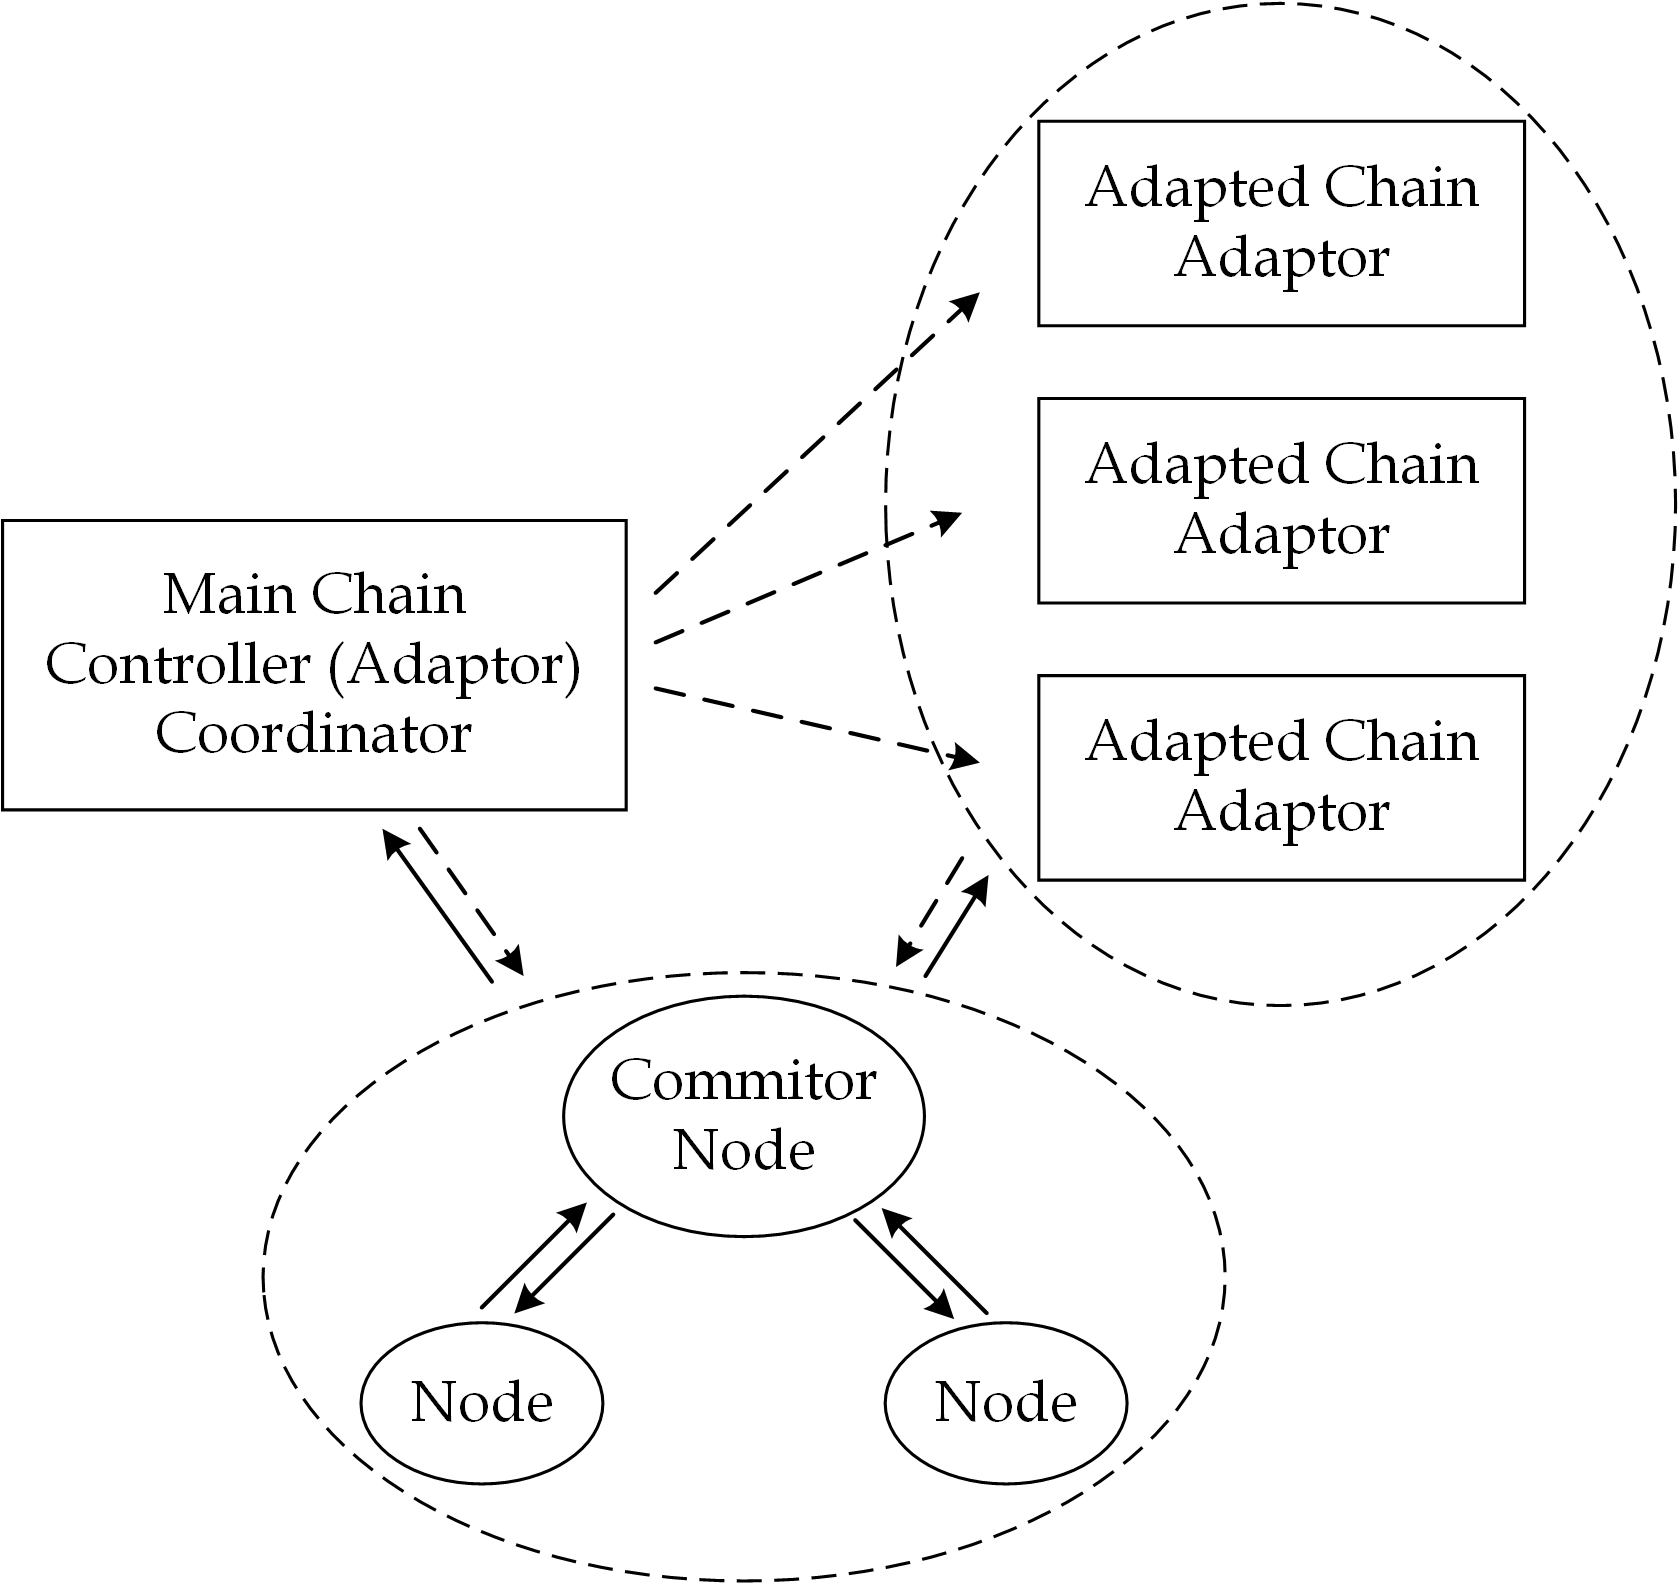
\includegraphics[width=0.5\textwidth]{figures/arpa network high level architecture.png}
    \caption{Caption}
    \label{fig:my_label}
\end{figure}

\section{Randcast}

The ARPA Network can be leveraged to build a variety of applications, distributed random number generator (DRNG) is one of them. Like the physical world, where the whole universe is built upon random motions of molecules, random numbers are ubiquitous and essential in the cyberspace. A trustworthy and reliable pseudo-random number generator is a cornerstone to either blockchain infrastructures or applications built upon. In this section, we instantiate Randcast as a randomness generation application of the ARPA Network.

An easy approach to achieve a random number is through a trusted third party. However, centralized randomness generation suffers a trust degradation with a concern for the backdoors. When used in a distributed system, a DRNG is desirable, and the threshold BLS signature is a cryptographic primitive to build one. Randcast leverages the ARPA Network to provide randomness service. Once the network receives a seed within a random number generation task. One group is called to generate a signature on the seed. The signature can then be used as a deterministic, verifiable, unforgeable random number. Inheriting from the threshold signature network, Randcast has the following features.

\begin{itemize}
    \item Decentralization, Randcast produces random numbers in a decentralized manner. Entropy is gathered from multiple entities located in different regions running individual nodes. This manner offers unpredictability and fairness in the physical level.
    \item Uniqueness, Randcast generates random numbers depending only on request messages and node secrets. Given certain signing group and user input, the randomness is unique and tamper-proof which mitigates corruption inside the network.
    \item Verifiability, Randcast allows everyone to check the validity of random number. By virtue of underlying cryptographic primitive, The random number is unlikely to be forged or manipulated
    \item Non-interactive, Randcast avoids heavy synchronous communication in the random generation phase. An non-interactive procedure guarantees a better service status.
    \item High availability, Randcast owns a high availability thanks to its decentralization and non-interactive. With the growth of its network size, the downtime will reduce accordingly.
    \item Multiple Chain Supported, Randcast is designed to adapt to multiple chains, facilitating developers from multiverse casting “randomness” spells. Our underlying threshold signature network will keep consistency between the different data replicas.
\end{itemize}

\appendix
\section{BLS 12-381 specification}
BLS12-381 is a specific curve of a pairing-friendly curve family. It has an embedded degree as 12 and a 381-bit field prime. The public parameters are outlined as follows\cite{sean2017bls}.

\begin{align*}
\texttt{u} &= \texttt{-0x} && \texttt{d2010000 00010000} \\
\texttt{k} &= &&\texttt{12} \\
\texttt{q} &= \texttt{ 0x} && \texttt{1a0111ea 397fe69a 4b1ba7b6 434bacd7 64774b84 f38512bf 6730d2a0} \\
& && \texttt{f6b0f624 1eabfffe b153ffff b9feffff ffffaaab} \\
\texttt{r} &= \texttt{ 0x} && \texttt{73eda753 299d7d48 3339d808 09a1d805 53bda402 fffe5bfe ffffffff}\\
& && \texttt{00000001} \\
\mathtt{E(\mathbb{F}_q)} &:= &&\mathtt{y^2 = x^3 + 4} \\
\mathtt{\mathbb{F}_{q^2}} &:= &&\mathtt{\mathbb{F}_q[i]/(x^2 + 1)} \\
\mathtt{E'(\mathbb{F}_{q^2})} &:= &&\mathtt{y^2 = x^3 + 4(i + 1)} \\
\end{align*}


\bibliographystyle{plain} % We choose the "plain" reference style
\bibliography{refs} % Entries are in the refs.bib file

\end{document}